% Biên dịch: xelatex -shell-escape main.tex (chạy 2 lần)
% Trên Overleaf: chọn compiler XeLaTeX hoặc pdfLaTeX đều được.
\documentclass[a4paper]{article}
\usepackage{iftex}
\ifXeTeX
  \usepackage{fontspec}
\else
  \usepackage{vntex}
\fi
\usepackage{a4wide,amssymb,latexsym,array,hhline,fancyhdr}
\usepackage{caption}
\usepackage{booktabs}
\usepackage{amsmath}
\usepackage{float}
\usepackage{lastpage}
\usepackage{graphicx}
\usepackage{tabularx}
\usepackage{multirow}
\usepackage{geometry}
\usepackage{setspace}
\usepackage{tikz}
\usetikzlibrary{arrows.meta,positioning,fit,shapes.geometric,calc}
\usepackage{hyperref}
% minted v3 cần latexminted, bản đi kèm Ubuntu bị lỗi với Python 3.14 nên ưu tiên minted2
\IfFileExists{minted2.sty}{\usepackage{minted2}}{\usepackage{minted}}
\usepackage{indentfirst}
\usepackage{xcolor}
\usepackage{longtable}
\usepackage[shortlabels]{enumitem}
\renewcommand{\baselinestretch}{1.4}
\hypersetup{urlcolor=blue,linkcolor=black,citecolor=black,colorlinks=true}

\setlength{\headheight}{40pt}
\pagestyle{fancy}
\fancyhead{}
\fancyhead[L]{
 \begin{tabular}{rl}
    \begin{picture}(25,15)(0,0)
    \put(0,-8){
\includegraphics[width=8mm, height=8mm]{images/khtn.png}}
    \end{picture}&
	\begin{tabular}{l}
		\textbf{\bf \ttfamily Trường đại học Khoa Học Tự Nhiên TP.HCM}\\
		\textbf{\bf \ttfamily Khoa Công Nghệ Thông Tin}
	\end{tabular}
 \end{tabular}
}
\fancyfoot{}
\fancyfoot[L]{\scriptsize \ttfamily Hệ điều hành -- Project 1: File \& Process Management}
\fancyfoot[R]{\scriptsize \ttfamily Trang {\thepage}/\pageref{LastPage}}
\renewcommand{\headrulewidth}{0.3pt}
\renewcommand{\footrulewidth}{0.3pt}

\setcounter{secnumdepth}{3}
\setcounter{tocdepth}{3}

%%% Khung code
\setminted{
  frame=single,
  bgcolor=lightgray!20,
  fontsize=\footnotesize,
  baselinestretch=1,
  breaklines=true,
  breakanywhere=true,
}

\newcommand{\cmd}[1]{\texttt{#1}}
\setlength{\emergencystretch}{3em}

\begin{document}

\begin{titlepage}
\begin{center}
ĐẠI HỌC QUỐC GIA THÀNH PHỐ HỒ CHÍ MINH\\
TRƯỜNG ĐẠI HỌC KHOA HỌC TỰ NHIÊN\\
KHOA CÔNG NGHỆ THÔNG TIN
\end{center}

\vspace{0.7cm}

\begin{figure}[h!]
\begin{center}

\includegraphics[width=5cm]{images/khtn.png}
\end{center}
\end{figure}

\vspace{0.5cm}

\begin{center}
\begin{tabular}{c}
\multicolumn{1}{c}{\textbf{{\normalsize HỆ ĐIỀU HÀNH}}}\\
~~\\
\hline
\\
\multicolumn{1}{l}{\textbf{{\Large Project 1}}}\\
\\
\textbf{{\Large FILE \& PROCESS MANAGEMENT TRÊN XV6}}\\
\\
\hline
\end{tabular}
\end{center}

\vspace{0.5cm}

\begin{table}[h]
\begin{tabular}{rrl}
\hspace{3.5cm} & Nhóm: & 6\\
\hspace{3.5cm} & Sinh viên thực hiện: & Nguyễn Quốc Đạt -- 24120282\\
\hspace{3.5cm} & & Nguyễn Thành Dự -- 24120288\\
\hspace{3.5cm} & & Nguyễn Đức Duy -- 24120294\\
\end{tabular}
\end{table}

\vspace{2.5cm}

\begin{center} {\footnotesize Thành phố Hồ Chí Minh, 11/2026}
\end{center}
\end{titlepage}

\thispagestyle{empty}

\newpage
\renewcommand{\contentsname}{Mục lục}
\renewcommand{\tablename}{Bảng}
\renewcommand{\figurename}{Hình}
\renewcommand{\refname}{Tài liệu tham khảo}
\tableofcontents

\newpage
\renewcommand{\arraystretch}{1.3}
\setcounter{page}{1}

\section{Tổng quan}

\subsection{Mức độ hoàn thành}

\begin{table}[H]
\centering
\small
\begin{tabularx}{\textwidth}{c >{\raggedright\arraybackslash}X c c}
\toprule
\textbf{STT} & \textbf{Yêu cầu} & \textbf{Mức độ} & \textbf{Mục} \\
\midrule
\multicolumn{4}{l}{\textit{4.1 -- Tìm hiểu và báo cáo}} \\
1 & Field \cmd{ofile[]} của \cmd{struct proc}, \cmd{file[]} của \cmd{struct ftable} & 100\% & \ref{sec:ofile-ftable} \\
2 & Trace system call \cmd{open} & 100\% & \ref{sec:trace-open} \\
3 & So sánh cách dùng file descriptor trong \cmd{open()}, \cmd{dup()}, \cmd{fork()} & 100\% & \ref{sec:compare-fd} \\
4 & Field \cmd{pid}, \cmd{state}, \cmd{context} của \cmd{struct proc} & 100\% & \ref{sec:proc-fields} \\
5 & Trace system call \cmd{fork} & 100\% & \ref{sec:trace-fork} \\
6 & Cơ chế lập lịch \cmd{scheduler()}, \cmd{sched()}, \cmd{yield()} & 100\% & \ref{sec:sched} \\
\midrule
\multicolumn{4}{l}{\textit{4.2 -- Cài đặt}} \\
7 & System call \cmd{sysinfo}: danh sách file đang mở & 100\% & \ref{sec:sysinfo} \\
8 & System call \cmd{sysinfo}: danh sách process khác \cmd{UNUSED} & 100\% & \ref{sec:sysinfo} \\
9 & Chương trình test \cmd{user/sysinfotest.c} (10 nhóm test) & 100\% & \ref{sec:testing} \\
\bottomrule
\end{tabularx}
\caption{Mức độ hoàn thành các yêu cầu}
\end{table}

Ngoài yêu cầu của đề, nhóm viết thêm lệnh \cmd{sysinfo} (\cmd{user/sysinfo.c})
để quan sát trạng thái hệ thống khi chạy các chương trình thật trong shell
(mục~\ref{sec:demo}).

\subsection{Phân công công việc}

\begin{table}[H]
\centering
\small
\begin{tabularx}{\textwidth}{l l X c}
\toprule
\textbf{MSSV} & \textbf{Họ tên} & \textbf{Công việc} & \textbf{Hoàn thành} \\
\midrule
24120282 & Nguyễn Quốc Đạt & \textit{(cần điền)} & 100\% \\
24120288 & Nguyễn Thành Dự & \textit{(cần điền)} & 100\% \\
24120294 & Nguyễn Đức Duy  & \textit{(cần điền)} & 100\% \\
\bottomrule
\end{tabularx}
\caption{Phân công công việc}
\end{table}

\subsection{Môi trường thực hiện}

\begin{itemize}
  \item Mã nguồn: xv6-labs-2024 (MIT 6.1810), nhánh \cmd{util}.
  \item Hệ điều hành: Ubuntu Linux; trình biên dịch \cmd{riscv64-linux-gnu-gcc};
        giả lập \cmd{qemu-system-riscv64} với 3 CPU (\cmd{-smp 3}).
  \item Biên dịch và chạy: \cmd{make qemu}; thoát QEMU bằng \cmd{Ctrl-a x}.
\end{itemize}

\section{Tìm hiểu về File}

\subsection{Field \texttt{ofile[]} của \texttt{struct proc} và \texttt{file[]} của \texttt{struct ftable}}
\label{sec:ofile-ftable}

File descriptor (fd) là một số nguyên nhỏ mà process dùng để chỉ tới một đối
tượng có thể đọc/ghi: file thường, thư mục, thiết bị (console) hoặc pipe.
Chương trình user chỉ thấy con số này; bên trong kernel, mỗi fd được giải mã
qua ba tầng (Hình~\ref{fig:fd-layers}).

\begin{figure}[H]
\centering
\begin{tikzpicture}[
  cell/.style={draw, minimum width=1.0cm, minimum height=0.55cm, font=\scriptsize\ttfamily},
  ent/.style={draw, minimum width=3.6cm, minimum height=0.55cm, font=\scriptsize\ttfamily, align=left, fill=blue!5},
  ino/.style={draw, rounded corners, minimum width=2.4cm, minimum height=0.55cm, font=\scriptsize\ttfamily, fill=green!8},
  ar/.style={-{Stealth[length=2mm]}, thick},
  ttl/.style={font=\small\bfseries}]
  % process A
  \node[ttl] at (0.5,0.7) {Process A};
  \foreach \i/\v in {0/fd 0,1/fd 1,2/fd 2,3/fd 3,4/fd 4}
    \node[cell] (a\i) at (0,-\i*0.55) {\v};
  \foreach \i in {0,...,4}
    \node[cell, right=0cm of a\i] (pa\i) {};
  % process B
  \node[ttl] at (0.5,-3.3) {Process B};
  \foreach \i/\v in {0/fd 0,1/fd 1,2/fd 2,3/fd 3}
    \node[cell] (b\i) at (0,-4.0-\i*0.55) {\v};
  \foreach \i in {0,...,3}
    \node[cell, right=0cm of b\i] (pb\i) {};
  % ftable
  \node[ttl] at (5.6,0.7) {ftable.file[NFILE]};
  \node[ent] (f0) at (5.6,-0.3)  {[0] DEVICE console\\\ \ \ \ ref=6 rw};
  \node[ent] (f1) at (5.6,-1.6)  {[1] INODE README\\\ \ \ \ ref=2 r- off=512};
  \node[ent] (f2) at (5.6,-2.9)  {[2] INODE README\\\ \ \ \ ref=1 r- off=0};
  \node[ent] (f3) at (5.6,-4.2)  {[3] (ref=0, trống)};
  % inodes
  \node[ttl] at (10.2,0.7) {inode (itable)};
  \node[ino] (i23) at (10.2,-0.3) {inode 23 (dev)};
  \node[ino] (i2)  at (10.2,-2.2) {inode 2 (file)};

  \draw[ar] (pa0.center) -- (f0.west);
  \draw[ar] (pa1.center) -- (f0.west);
  \draw[ar] (pa2.center) -- (f0.west);
  \draw[ar] (pa3.center) -- (f1.west);
  \draw[ar] (pa4.center) -- (f2.west);
  \draw[ar] (pb0.center) -- (f0.west);
  \draw[ar] (pb1.center) -- (f0.west);
  \draw[ar] (pb2.center) -- (f0.west);
  \draw[ar] (pb3.center) -- (f1.west);
  \draw[ar] (f0.east) -- (i23.west);
  \draw[ar] (f1.east) -- (i2.west);
  \draw[ar] (f2.east) -- (i2.west);

  \node[font=\scriptsize, align=center] at (0.5,-6.5) {p->ofile[NOFILE]\\(riêng từng process)};
  \node[font=\scriptsize, align=center] at (5.6,-6.5) {struct file\\(dùng chung toàn hệ thống)};
  \node[font=\scriptsize, align=center] at (10.2,-6.5) {struct inode\\(file thật)};
\end{tikzpicture}
\caption{Ba tầng giải mã file descriptor. B là con của A, được tạo bằng
\texttt{fork} sau khi A mở README lần thứ nhất (fd 3) nên dùng chung ô [1]; sau
đó A mở README lần nữa (fd 4) và nhận ô [2] riêng.}
\label{fig:fd-layers}
\end{figure}

\paragraph{\texttt{p->ofile[NOFILE]}.}
Mảng 16 con trỏ \cmd{struct file*} trong \cmd{struct proc}; \textbf{fd chính
là chỉ số} trong mảng này. Ô bằng 0 nghĩa là fd đó chưa dùng. Mảng là riêng
của từng process, nên fd 3 của process A và fd 3 của process B có thể trỏ tới
hai file khác nhau. Theo quy ước, fd 0, 1, 2 là stdin, stdout, stderr. Field
này thuộc nhóm ``riêng tư'' của \cmd{struct proc}, chỉ chính process đó
sửa (trong \cmd{open}, \cmd{dup}, \cmd{close}, \cmd{fork}, \cmd{exit}) nên
không cần \cmd{p->lock}.

\paragraph{\texttt{ftable.file[NFILE]}.}
Bảng file đang mở của toàn hệ thống (\cmd{kernel/file.c}), gồm 100 phần tử
\cmd{struct file} và một spinlock \cmd{ftable.lock}. Mỗi phần tử ứng với
\emph{một lần mở} (một lần gọi \cmd{open} hoặc \cmd{pipe}):

\begin{table}[H]
\centering
\small
\begin{tabularx}{\textwidth}{>{\ttfamily}l X}
\toprule
\textrm{\textbf{Field}} & \textbf{Ý nghĩa} \\
\midrule
type & \cmd{FD\_NONE} (ô trống), \cmd{FD\_PIPE}, \cmd{FD\_INODE} (file, thư mục),
       \cmd{FD\_DEVICE} (thiết bị như console). \\
ref & Số con trỏ đang trỏ vào ô này (từ \cmd{ofile[]} của mọi process).
      \cmd{ref == 0} nghĩa là ô trống. Được bảo vệ bởi \cmd{ftable.lock}. \\
readable, writable & Mode mở: được đọc / được ghi hay không. \\
pipe & Con trỏ tới \cmd{struct pipe} nếu là pipe. \\
ip & Con trỏ tới inode nếu là file, thư mục hoặc thiết bị. \\
off & Vị trí đọc/ghi hiện tại (chỉ với \cmd{FD\_INODE}). \\
major & Số hiệu thiết bị (chỉ với \cmd{FD\_DEVICE}), dùng tra bảng \cmd{devsw[]}. \\
\bottomrule
\end{tabularx}
\caption{Các field của \texttt{struct file}}
\end{table}

Các hàm quản lý bảng:
\begin{itemize}
  \item \cmd{filealloc()}: dưới \cmd{ftable.lock}, tìm ô có \cmd{ref == 0},
        đặt \cmd{ref = 1} và trả về ô đó.
  \item \cmd{filedup(f)}: tăng \cmd{f->ref}.
  \item \cmd{fileclose(f)}: giảm \cmd{f->ref}; khi về 0 thì đặt
        \cmd{type = FD\_NONE} và giải phóng tài nguyên bên dưới
        (\cmd{pipeclose} hoặc \cmd{iput}).
\end{itemize}

\paragraph{Vì sao cần tầng \texttt{ftable} ở giữa.}
Nếu \cmd{ofile[]} trỏ thẳng vào inode thì không có chỗ lưu offset riêng cho
từng lần mở. Tầng \cmd{struct file} cho phép offset vừa được \emph{chia sẻ}
(giữa các fd tạo bởi \cmd{dup} hoặc \cmd{fork}) vừa được \emph{tách biệt}
(giữa hai lần \cmd{open} khác nhau trên cùng một file).

\subsection{Trace system call \texttt{open}}
\label{sec:trace-open}

\begin{enumerate}
  \item \textbf{User space:} \cmd{open(path, omode)} nạp \cmd{SYS\_open} vào
        \cmd{a7}, gọi \cmd{ecall}. Kernel đi qua \cmd{uservec}
        $\to$ \cmd{usertrap()} $\to$ \cmd{syscall()} $\to$ \cmd{sys\_open()}
        (\cmd{kernel/sysfile.c}), giống như \cmd{fork} ở mục~\ref{sec:trace-fork}.
  \item \textbf{Lấy tham số:} \cmd{argint(1, \&omode)} lấy mode;
        \cmd{argstr(0, path, MAXPATH)} chép chuỗi đường dẫn từ bộ nhớ user vào
        kernel (qua \cmd{copyinstr}, dùng page table của process).
  \item \textbf{Bắt đầu transaction:} \cmd{begin\_op()}, vì \cmd{open} có thể
        ghi lên đĩa (tạo file mới).
  \item \textbf{Tìm hoặc tạo inode:}
        \begin{itemize}
          \item Có \cmd{O\_CREATE}: \cmd{create(path, T\_FILE, 0, 0)} tìm thư
                mục cha, nếu file chưa có thì \cmd{ialloc} một inode mới và
                \cmd{dirlink} thêm entry vào thư mục. Trả về inode đã khóa.
          \item Không có \cmd{O\_CREATE}: \cmd{namei(path)} duyệt đường dẫn
                từng thành phần (\cmd{dirlookup}) để lấy inode, rồi
                \cmd{ilock(ip)} (đọc inode từ đĩa nếu chưa có trong bộ nhớ).
                Nếu là thư mục mà mở để ghi thì trả về lỗi.
        \end{itemize}
  \item \textbf{Kiểm tra thiết bị:} nếu \cmd{T\_DEVICE} thì \cmd{major} phải
        hợp lệ ($0 \le \text{major} < \text{NDEV}$).
  \item \textbf{Cấp \texttt{struct file}:} \cmd{filealloc()} lấy một ô trống
        trong \cmd{ftable} (\cmd{ref = 1}). Nếu bảng đầy (100 ô), trả về $-1$.
  \item \textbf{Cấp fd:} \cmd{fdalloc(f)} duyệt \cmd{p->ofile[]} từ 0, gán
        \cmd{f} vào \textbf{ô trống có chỉ số nhỏ nhất} và trả về chỉ số đó.
        Nếu process đã dùng đủ 16 fd, \cmd{fileclose(f)} trả lại ô
        \cmd{ftable} và \cmd{open} trả về $-1$.
  \item \textbf{Điền \texttt{struct file}:} \cmd{type} là \cmd{FD\_DEVICE}
        (kèm \cmd{major}) hoặc \cmd{FD\_INODE} (kèm \cmd{off = 0});
        \cmd{ip = ip}; \cmd{readable = !(omode \& O\_WRONLY)};
        \cmd{writable = (omode \& O\_WRONLY) || (omode \& O\_RDWR)}.
  \item \textbf{\texttt{O\_TRUNC}:} nếu có và là file thường thì
        \cmd{itrunc(ip)} xóa nội dung.
  \item \textbf{Kết thúc:} \cmd{iunlock(ip)} (vẫn giữ tham chiếu inode qua
        \cmd{f->ip}), \cmd{end\_op()}, trả về \cmd{fd}.
\end{enumerate}

Bước 7 (chọn fd nhỏ nhất) là cơ sở của chuyển hướng I/O trong shell: với lệnh
\cmd{sysinfo -f > out}, shell \cmd{close(1)} rồi \cmd{open("out", ...)}, nên
file \cmd{out} nhận đúng fd 1 (kết quả ở Hình~\ref{fig:demo-redirect}).

\subsection{So sánh cách dùng file descriptor trong \texttt{open()}, \texttt{dup()}, \texttt{fork()}}
\label{sec:compare-fd}

\begin{table}[H]
\centering
\small
\begin{tabularx}{\textwidth}{>{\raggedright\arraybackslash}p{3.0cm} X X X}
\toprule
 & \cmd{open(path, mode)} & \cmd{dup(fd)} & \cmd{fork()} \\
\midrule
fd mới & 1 fd, nhỏ nhất còn trống & 1 fd, nhỏ nhất còn trống
       & Process con có bản sao toàn bộ \cmd{ofile[]}, cùng số fd \\
\cmd{struct file} & \textbf{Cấp ô mới} (\cmd{filealloc}) & Dùng lại ô cũ
       & Dùng lại các ô của cha \\
\cmd{ref} & Ô mới có \cmd{ref = 1} & \cmd{ref + 1}
          & Mỗi ô đang mở: \cmd{ref + 1} (\cmd{filedup}) \\
Offset & Riêng, bắt đầu từ 0 & Dùng chung với fd gốc & Dùng chung giữa cha và con \\
Mode & Theo tham số \cmd{mode} & Giống fd gốc & Giống của cha \\
Phạm vi & Trong process gọi & Trong process gọi & Giữa hai process \\
Ứng dụng & Mở file & Chuyển hướng I/O, ví dụ \cmd{init} tạo fd 1, 2 từ fd 0
         & Shell chia sẻ console và pipe cho lệnh con \\
\bottomrule
\end{tabularx}
\caption{So sánh file descriptor trong \texttt{open}, \texttt{dup}, \texttt{fork}}
\end{table}

Tóm lại, chỉ \cmd{open} (và \cmd{pipe}) tạo ra một \cmd{struct file} mới.
\cmd{dup} và \cmd{fork} chỉ tạo thêm con trỏ tới \cmd{struct file} đã có, nên
các fd đó \emph{dùng chung offset}: ví dụ cha và con cùng ghi vào một file sau
\cmd{fork} thì dữ liệu được nối tiếp chứ không ghi đè lên nhau. Ngược lại, hai
lần \cmd{open} cùng một file cho hai \cmd{struct file} độc lập, chỉ dùng chung
inode.

Các tính chất này được kiểm chứng bằng \cmd{sysinfo} trong test
\cmd{test\_openclose}, \cmd{test\_dup}, \cmd{test\_fork}
(mục~\ref{sec:testing}): hai lần \cmd{open} cho hai \cmd{idx} khác nhau cùng
\cmd{inum}; \cmd{dup} cho cùng \cmd{idx} với \cmd{ref = 3} và offset chung;
sau \cmd{fork} các fd của con có cùng \cmd{idx} với cha và \cmd{ref} tăng 1.

\section{Tìm hiểu về Process}

\subsection{Khái niệm process trong xv6}

Process là \emph{đơn vị cách ly} của xv6: một process không
thể đọc hay phá bộ nhớ, CPU, file descriptor của process khác, cũng không thể
phá kernel. Để làm được điều này, kernel tạo cho mỗi chương trình hai ảo giác:

\begin{itemize}
  \item \textbf{Bộ nhớ riêng (address space):} mỗi process có một page table
        riêng (\cmd{p->pagetable}) ánh xạ địa chỉ ảo bắt đầu từ 0 sang bộ nhớ
        vật lý. Process này không nhìn thấy bộ nhớ của process khác.
  \item \textbf{CPU riêng (thread):} kernel luân phiên CPU giữa các process.
        Khi một process không chạy, các thanh ghi của nó được lưu lại và khôi
        phục khi nó được chạy tiếp.
\end{itemize}

Trong xv6 mỗi process có đúng một address space và một thread. Mỗi process có
\textbf{hai stack}: user stack dùng khi chạy code user và kernel stack
(\cmd{p->kstack}, 1 trang) dùng khi vào kernel qua system call hoặc
interrupt. Kernel stack được tách riêng và được bảo vệ để kernel vẫn chạy
đúng kể cả khi chương trình user làm hỏng user stack của nó.

Kernel quản lý process bằng một mảng cố định \cmd{struct proc proc[NPROC]}
(\cmd{NPROC = 64}). Không có cấp phát động: tạo process nghĩa là tìm một ô
có \cmd{state == UNUSED} và điền thông tin vào (\cmd{allocproc()}).

\subsection{Các field \texttt{pid}, \texttt{state}, \texttt{context} của \texttt{struct proc}}
\label{sec:proc-fields}

\cmd{struct proc} (\cmd{kernel/proc.h}) chứa toàn bộ trạng thái kernel của
một process. Các field được chia nhóm theo khóa bảo vệ chúng
(Bảng~\ref{tab:proc-groups}).

\begin{table}[H]
\centering
\small
\begin{tabularx}{\textwidth}{>{\raggedright\arraybackslash}p{3.3cm} >{\raggedright\arraybackslash}p{4.3cm} X}
\toprule
\textbf{Khóa bảo vệ} & \textbf{Field} & \textbf{Lý do} \\
\midrule
\cmd{p->lock} & \cmd{state}, \cmd{pid}, \cmd{chan}, \cmd{killed}, \cmd{xstate}
  & Được process khác và scheduler trên CPU khác đọc/ghi. \\
\cmd{wait\_lock} (toàn cục) & \cmd{parent}
  & Process chưa biết cha mình là ai cho tới khi lấy được khóa, nên không thể
    dùng khóa riêng của cha. \\
Không cần khóa & \cmd{kstack}, \cmd{sz}, \cmd{pagetable}, \cmd{trapframe},
  \cmd{context}, \cmd{ofile}, \cmd{cwd}, \cmd{name}
  & Chỉ chính process đó sử dụng. \\
\bottomrule
\end{tabularx}
\caption{Các nhóm field của \texttt{struct proc}}
\label{tab:proc-groups}
\end{table}

\subsubsection{\texttt{pid} -- định danh process}

\cmd{pid} là số nguyên dương duy nhất, cấp bởi \cmd{allocpid()} khi
\cmd{allocproc()} tìm được ô trống. Hàm này tăng biến toàn cục \cmd{nextpid}
dưới khóa \cmd{pid\_lock}, nên hai CPU tạo process cùng lúc không bao giờ nhận
trùng pid. Process đầu tiên (\cmd{init}) có pid 1. pid không được tái sử dụng
dù ô \cmd{proc[]} có được dùng lại.

pid được dùng làm giá trị trả về của \cmd{fork()} cho process cha, giá trị trả
về của \cmd{wait()}, và tham số của \cmd{kill(pid)}. Vì \cmd{kill} và
\cmd{wait} đọc pid của process khác nên field này phải được bảo vệ bởi
\cmd{p->lock}: \cmd{kill} cần chắc chắn process nạn nhân không thoát và bị
cấp phát lại giữa lúc kiểm tra pid và lúc đặt cờ \cmd{killed}.

\subsubsection{\texttt{state} -- trạng thái process}

\cmd{state} có kiểu
\cmd{enum procstate \{UNUSED, USED, SLEEPING, RUNNABLE, RUNNING, ZOMBIE\}},
cho biết ô trong bảng đang trống, đang được dựng, đang chờ sự kiện, sẵn sàng
chạy, đang chạy trên một CPU, hay đã kết thúc nhưng chưa được cha thu dọn.
Hình~\ref{fig:state} và Bảng~\ref{tab:state} mô tả các chuyển trạng thái.

\begin{figure}[H]
\centering
\begin{tikzpicture}[
  st/.style={draw, rounded corners, minimum width=2.3cm, minimum height=0.9cm,
             font=\small\ttfamily, fill=blue!6},
  ar/.style={-{Stealth[length=2.5mm]}, thick},
  lb/.style={font=\scriptsize, fill=white, inner sep=1pt},
  node distance=1.3cm and 2.2cm]
  \node[st] (unused) {UNUSED};
  \node[st, right=of unused] (used) {USED};
  \node[st, right=of used] (runnable) {RUNNABLE};
  \node[st, below=1.9cm of runnable] (running) {RUNNING};
  \node[st, below=1.9cm of used] (sleeping) {SLEEPING};
  \node[st, below=1.9cm of unused] (zombie) {ZOMBIE};

  \draw[ar] (unused) -- node[lb, above]{allocproc} (used);
  \draw[ar] (used) -- node[lb, above]{fork/userinit} (runnable);
  \draw[ar] ([xshift=-4mm]runnable.south) -- node[lb, left]{scheduler} ([xshift=-4mm]running.north);
  \draw[ar] ([xshift=4mm]running.north) -- node[lb, right]{yield} ([xshift=4mm]runnable.south);
  \draw[ar] (running) -- node[lb, below]{sleep} (sleeping);
  \draw[ar] (sleeping) -- node[lb, above, sloped]{wakeup} (runnable);
  \draw[ar] (running.south) -- ++(0,-0.6) -| node[lb, pos=0.25, below]{exit} (zombie.south);
  \draw[ar] (zombie) -- node[lb, left]{wait (cha) + freeproc} (unused);
\end{tikzpicture}
\caption{Sơ đồ chuyển trạng thái của process trong xv6}
\label{fig:state}
\end{figure}

\begin{table}[H]
\centering
\small
\begin{tabularx}{\textwidth}{>{\ttfamily}l X}
\toprule
\textrm{\textbf{Chuyển}} & \textbf{Nguyên nhân} \\
\midrule
UNUSED $\to$ USED & \cmd{allocproc()} tìm thấy ô trống: gán pid, cấp trang
  trapframe, tạo page table, đặt \cmd{context.ra = forkret}. \\
USED $\to$ RUNNABLE & Cuối \cmd{fork()} (hoặc \cmd{userinit()}), sau khi đã
  dựng xong toàn bộ process con. \\
RUNNABLE $\to$ RUNNING & \cmd{scheduler()} chọn process để chạy. \\
RUNNING $\to$ RUNNABLE & \cmd{yield()}: hết lượt do timer interrupt. \\
RUNNING $\to$ SLEEPING & \cmd{sleep(chan)}: chờ sự kiện (đọc pipe, \cmd{wait},
  đọc console, \ldots); \cmd{p->chan} ghi lại kênh đang chờ. \\
SLEEPING $\to$ RUNNABLE & \cmd{wakeup(chan)} từ process khác hoặc interrupt. \\
RUNNING $\to$ ZOMBIE & \cmd{exit()}: đóng file, giao con cho \cmd{init},
  đánh thức cha, lưu \cmd{xstate}. \\
ZOMBIE $\to$ UNUSED & \cmd{wait()} của cha lấy mã thoát rồi gọi
  \cmd{freeproc()}. \\
\bottomrule
\end{tabularx}
\caption{Các chuyển trạng thái và hàm gây ra chúng}
\label{tab:state}
\end{table}

Trạng thái \cmd{ZOMBIE} cần thiết vì hai lý do: process cha
có thể chưa gọi \cmd{wait} khi con thoát nên kernel phải giữ lại mã thoát;
và một process không thể tự giải phóng kernel stack mà nó đang chạy trên đó.
Nếu cha thoát trước con, \cmd{exit()} gọi \cmd{reparent()} để giao các con
cho \cmd{init}, process luôn gọi \cmd{wait} trong vòng lặp, nên mọi process
con đều có người thu dọn.

Trạng thái \cmd{USED} là trạng thái trung gian khi process đang được dựng.
Scheduler chỉ chạy process \cmd{RUNNABLE}, nên một process đang dựng dở bị
``che'' khỏi scheduler cho tới khi \cmd{fork()} đặt nó thành \cmd{RUNNABLE}
ở bước cuối cùng.

\subsubsection{\texttt{context} -- ngữ cảnh kernel thread}

\cmd{struct context} lưu 14 thanh ghi của \emph{kernel thread} của process:
\cmd{ra}, \cmd{sp} và các thanh ghi callee-saved \cmd{s0}--\cmd{s11}. Nó
được dùng bởi hàm assembly \cmd{swtch(old, new)} (\cmd{kernel/swtch.S}):
lưu các thanh ghi hiện tại vào \cmd{old}, nạp các thanh ghi từ \cmd{new},
rồi \cmd{ret}.

\begin{itemize}
  \item \cmd{swtch} chỉ lưu các thanh ghi callee-saved, vì trình biên dịch C đã
        lưu các thanh ghi caller-saved lên stack trước khi gọi hàm.
  \item \cmd{swtch} không lưu \cmd{pc}, mà lưu \cmd{ra}. Khi \cmd{ret}, CPU nhảy tới \cmd{ra} vừa
        nạp, tức là ngay sau lệnh gọi \cmd{swtch} trước đây của thread kia.
  \item Vì \cmd{sp} cũng được nạp lại, CPU chuyển sang chạy trên stack của
        thread kia.
\end{itemize}

Mỗi CPU cũng có một \cmd{context} trong \cmd{struct cpu}, là ngữ cảnh của
\emph{scheduler thread} của CPU đó. Process chuyển CPU bằng
\cmd{swtch(\&p->context, \&mycpu()->context)} và scheduler chuyển CPU cho
process bằng \cmd{swtch(\&c->context, \&p->context)}.

Cần phân biệt \cmd{context} với \cmd{trapframe} (Bảng~\ref{tab:ctx-tf}):

\begin{table}[H]
\centering
\small
\begin{tabularx}{\textwidth}{l X X}
\toprule
 & \cmd{p->trapframe} & \cmd{p->context} \\
\midrule
Lưu gì & Toàn bộ thanh ghi \emph{user} (\cmd{epc}, \cmd{sp}, \cmd{a0}--\cmd{a7}, \ldots)
       & \cmd{ra}, \cmd{sp}, \cmd{s0}--\cmd{s11} của \emph{kernel thread} \\
Khi nào & User $\to$ kernel (system call, interrupt)
        & Kernel thread $\to$ scheduler (\cmd{swtch}) \\
Ai lưu & \cmd{uservec} trong \cmd{trampoline.S} & \cmd{swtch.S} \\
Mục đích & Quay về đúng lệnh trong chương trình user
         & Quay về đúng chỗ trong code kernel \\
\bottomrule
\end{tabularx}
\caption{So sánh \texttt{trapframe} và \texttt{context}}
\label{tab:ctx-tf}
\end{table}

Khi \cmd{allocproc()} tạo process mới, nó đặt \cmd{context.ra = forkret} và
\cmd{context.sp = p->kstack + PGSIZE}. Do đó lần đầu scheduler \cmd{swtch} vào
process mới, CPU ``quay về'' đầu hàm \cmd{forkret()} trên kernel stack rỗng
của process đó.

\subsection{Trace system call \texttt{fork}}
\label{sec:trace-fork}

\subsubsection{Từ user vào kernel}

\begin{enumerate}
  \item Chương trình user gọi \cmd{fork()}. Hàm này được sinh bởi
        \cmd{user/usys.pl}: nạp số hiệu \cmd{SYS\_fork} vào thanh ghi \cmd{a7}
        rồi thực thi lệnh \cmd{ecall}.
  \item \cmd{ecall} chuyển CPU sang supervisor mode và nhảy tới \cmd{uservec}
        (\cmd{kernel/trampoline.S}). \cmd{uservec} lưu toàn bộ thanh ghi user
        vào \cmd{p->trapframe}, chuyển sang page table kernel và kernel stack
        của process, rồi gọi \cmd{usertrap()}.
  \item \cmd{usertrap()} (\cmd{kernel/trap.c}) thấy \cmd{scause == 8}
        (system call), tăng \cmd{trapframe->epc} thêm 4 để khi trở về sẽ chạy
        lệnh sau \cmd{ecall}, bật interrupt và gọi \cmd{syscall()}.
  \item \cmd{syscall()} đọc \cmd{a7}, tra bảng \cmd{syscalls[]} và gọi
        \cmd{sys\_fork()}, hàm này chỉ gọi \cmd{fork()} trong \cmd{kernel/proc.c}.
        Giá trị trả về được ghi vào \cmd{trapframe->a0}.
\end{enumerate}

\subsubsection{Hàm \texttt{fork()} trong kernel}

\begin{enumerate}
  \item \textbf{Cấp phát process:} \cmd{allocproc()} duyệt \cmd{proc[]}, tìm
        ô \cmd{UNUSED}, gán pid mới, chuyển sang \cmd{USED}, cấp trang
        trapframe, tạo page table rỗng (chỉ có trampoline và trapframe) và
        khởi tạo \cmd{context}. Hàm trả về với \cmd{np->lock} đang được giữ.
        Nếu hết ô hoặc hết bộ nhớ, \cmd{fork} trả về $-1$.
  \item \textbf{Sao chép bộ nhớ:} \cmd{uvmcopy()} cấp trang mới và chép toàn
        bộ bộ nhớ user (code, data, stack, heap) của cha sang con, rồi đặt
        \cmd{np->sz = p->sz}. Hai process có nội dung bộ nhớ giống nhau nhưng
        nằm ở các trang vật lý khác nhau.
  \item \textbf{Sao chép thanh ghi user:} \cmd{*(np->trapframe) = *(p->trapframe)}.
        Do đó khi con trở về user space, nó tiếp tục chạy ngay sau lệnh
        \cmd{ecall} của \cmd{fork}, giống hệt cha.
  \item \textbf{Giá trị trả về của con:} \cmd{np->trapframe->a0 = 0}. Đây là
        điểm khác duy nhất giữa thanh ghi của cha và con, giải thích vì sao
        \cmd{fork} ``trả về hai lần'': 0 ở con, pid của con ở cha.
  \item \textbf{Chia sẻ file đang mở:} với mỗi \cmd{p->ofile[i]} khác 0,
        gán \cmd{np->ofile[i]} bằng \cmd{filedup(p->ofile[i])}. \cmd{filedup} chỉ tăng
        \cmd{ref} của \cmd{struct file} chứ không mở file mới, nên cha và con
        dùng chung offset. Thư mục hiện tại được chia sẻ bằng \cmd{idup(p->cwd)}.
  \item \textbf{Tên:} chép \cmd{p->name} sang \cmd{np->name}.
  \item \textbf{Ghi nhận cha:} nhả \cmd{np->lock}, lấy \cmd{wait\_lock}, đặt
        \cmd{np->parent = p}.
  \item \textbf{Cho phép chạy:} lấy lại \cmd{np->lock}, đặt
        \cmd{np->state = RUNNABLE}. Chỉ từ lúc này scheduler mới có thể chọn
        process con.
  \item Trả về pid của con. Giá trị này đi qua \cmd{trapframe->a0} của cha.
\end{enumerate}

\subsubsection{Lần chạy đầu tiên của process con}

Khi một CPU chọn process con, \cmd{scheduler()} gọi
\cmd{swtch(\&c->context, \&np->context)}. Vì \cmd{context.ra = forkret}, CPU
nhảy vào \cmd{forkret()}. Hàm này nhả \cmd{p->lock} (khóa được scheduler lấy
trước khi \cmd{swtch}, xem mục~\ref{sec:lock-swtch}), lần đầu tiên thì khởi
tạo file system, rồi gọi \cmd{usertrapret()}. \cmd{usertrapret()} và
\cmd{userret} nạp lại thanh ghi user từ trapframe đã sao chép ở bước 3 và
thực thi \cmd{sret}. Process con trở về user space ngay sau lệnh \cmd{ecall},
với \cmd{a0 = 0}.

Process cha trở về theo đường bình thường: \cmd{syscall()} ghi pid vào
\cmd{a0}, \cmd{usertrap()} gọi \cmd{usertrapret()} và cha tiếp tục chạy. Thứ
tự cha hay con chạy trước phụ thuộc vào scheduler.

\subsection{Cơ chế lập lịch: \texttt{scheduler()}, \texttt{sched()}, \texttt{yield()}}
\label{sec:sched}

\subsubsection{Khi nào CPU chuyển sang process khác}

xv6 chuyển process trong hai trường hợp:
\begin{itemize}
  \item \textbf{Tự nguyện:} process gọi một system call phải chờ (\cmd{read},
        \cmd{wait}, \cmd{sleep}, \ldots) và đi vào \cmd{sleep()}.
  \item \textbf{Bắt buộc:} timer interrupt định kỳ. Khi \cmd{devintr()} trả
        về 2 (timer), \cmd{usertrap()} hoặc \cmd{kerneltrap()} gọi
        \cmd{yield()}, ép process đang tính toán nhường CPU.
\end{itemize}

\subsubsection{\texttt{scheduler()}}

Mỗi CPU, sau khi khởi động xong, gọi \cmd{scheduler()} và không bao giờ
quay lại. Hàm này là một vòng lặp vô hạn chạy trên stack riêng của CPU
(scheduler thread):

\begin{enumerate}
  \item Bật interrupt (tránh deadlock khi mọi process đều đang chờ I/O).
  \item Duyệt lần lượt \cmd{proc[0..NPROC-1]}. Với mỗi \cmd{p}: lấy
        \cmd{p->lock}; nếu \cmd{p->state == RUNNABLE} thì đặt
        \cmd{p->state = RUNNING}, \cmd{c->proc = p}, rồi
        \cmd{swtch(\&c->context, \&p->context)} để chạy \cmd{p}.
  \item Khi \cmd{p} nhường CPU, \cmd{swtch} ``trả về'' trong scheduler. Đặt
        \cmd{c->proc = 0}, nhả \cmd{p->lock} và xét process tiếp theo.
  \item Nếu duyệt hết bảng mà không có process nào \cmd{RUNNABLE}, CPU thực thi
        \cmd{wfi} để nghỉ tới interrupt tiếp theo.
\end{enumerate}

Chính sách này là \textbf{round robin}: các process được chạy lần lượt,
không có độ ưu tiên. Scheduler chạy trên stack riêng thay vì
stack của một process, vì nếu dùng stack của process thì process đó có thể
được đánh thức và chạy trên CPU khác, dẫn tới hai CPU dùng chung một stack.

\subsubsection{\texttt{sched()}}

\cmd{sched()} là \emph{điểm duy nhất} một kernel thread nhường CPU cho
scheduler. Trước khi gọi \cmd{swtch(\&p->context, \&mycpu()->context)}, nó
kiểm tra bốn điều kiện, vi phạm bất kỳ điều kiện nào sẽ gây \cmd{panic}:
\begin{itemize}
  \item đang giữ \cmd{p->lock};
  \item chỉ giữ đúng một khóa (\cmd{mycpu()->noff == 1}), vì giữ thêm khóa
        khác qua \cmd{swtch} có thể gây deadlock;
  \item \cmd{p->state != RUNNING}, tức là người gọi đã đổi trạng thái;
  \item interrupt đang tắt.
\end{itemize}
\cmd{sched()} cũng lưu và khôi phục \cmd{intena}, vì đây là thuộc tính của
kernel thread chứ không phải của CPU. Mọi nơi muốn nhường CPU (\cmd{yield},
\cmd{sleep}, \cmd{exit}) đều làm theo cùng một mẫu: lấy \cmd{p->lock}, đổi
\cmd{p->state}, gọi \cmd{sched()}.

\subsubsection{\texttt{yield()}}

\cmd{yield()} là cách nhường CPU khi hết lượt: lấy \cmd{p->lock}, đặt
\cmd{p->state = RUNNABLE}, gọi \cmd{sched()}. Khi process được chọn chạy lại,
\cmd{sched()} trả về và \cmd{yield()} nhả \cmd{p->lock}. Process ở trạng
thái \cmd{RUNNABLE} nên sẽ được scheduler chọn lại ở một vòng duyệt sau.

\subsubsection{Toàn bộ quá trình chuyển process}

Hình~\ref{fig:switch} mô tả việc
chuyển từ process \cmd{shell} sang process \cmd{cat} trên một CPU. Mỗi lần
chuyển gồm \textbf{hai} lần \cmd{swtch}: process $\to$ scheduler và
scheduler $\to$ process mới. \cmd{sched} và \cmd{scheduler} luân phiên
chuyển quyền điều khiển cho nhau, nên chúng được gọi là các \emph{coroutine}.

\begin{figure}[H]
\centering
\begin{tikzpicture}[
  box/.style={draw, rounded corners, font=\scriptsize\ttfamily, align=center,
              minimum height=0.75cm, fill=blue!5},
  ar/.style={-{Stealth[length=2mm]}, thick},
  lb/.style={font=\scriptsize, align=center}]
  % user / kernel boundary
  \draw[dashed, gray] (-1.2,0) -- (13.2,0);
  \node[font=\scriptsize, gray] at (6,0.25) {user space};
  \node[font=\scriptsize, gray] at (6,-0.25) {kernel space};

  \node[box, fill=green!8] (sh) at (0,1.1) {shell\\(user)};
  \node[box] (ut) at (0,-1.2) {usertrap};
  \node[box] (y) at (0,-2.5) {yield\\sched};
  \node[box, fill=orange!12] (sc) at (6,-2.5) {scheduler\\(stack CPU)};
  \node[box] (s2) at (12,-2.5) {sched\\yield};
  \node[box] (ur) at (12,-1.2) {usertrapret};
  \node[box, fill=green!8] (cat) at (12,1.1) {cat\\(user)};

  \draw[ar] (sh) -- node[lb, right, pos=0.25, fill=white]{timer interrupt} (ut);
  \draw[ar] (ut) -- (y);
  \draw[ar] (y) -- node[lb, above]{swtch(\&shell->context,\\\&cpu->context)} (sc);
  \draw[ar] (sc) -- node[lb, above]{swtch(\&cpu->context,\\\&cat->context)} (s2);
  \draw[ar] (s2) -- (ur);
  \draw[ar] (ur) -- node[lb, left, pos=0.75, fill=white]{sret} (cat);

  \node[lb, below=0.15cm of y] {kstack shell};
  \node[lb, below=0.15cm of sc] {release(shell->lock)\\acquire(cat->lock)};
  \node[lb, below=0.15cm of s2] {kstack cat};
\end{tikzpicture}
\caption{Chuyển CPU từ \texttt{shell} sang \texttt{cat}}
\label{fig:switch}
\end{figure}

\subsubsection{Khóa \texttt{p->lock} được giữ qua \texttt{swtch}}
\label{sec:lock-swtch}

Thông thường thread nào lấy khóa thì chính thread đó nhả khóa. Trong xv6,
\cmd{p->lock} được giữ xuyên qua \cmd{swtch}:
\begin{itemize}
  \item \cmd{yield()} của \cmd{shell} lấy \cmd{shell->lock}, nhưng
        \cmd{scheduler()} mới là nơi nhả nó.
  \item \cmd{scheduler()} lấy \cmd{cat->lock}, nhưng \cmd{yield()} của
        \cmd{cat} (hoặc \cmd{forkret()} nếu \cmd{cat} vừa được tạo) mới nhả nó.
\end{itemize}
Lý do: nếu \cmd{shell->lock} được nhả ngay sau khi đặt
\cmd{state = RUNNABLE} nhưng trước khi \cmd{swtch} lưu xong ngữ cảnh, scheduler
của một CPU khác có thể chọn \cmd{shell} và chạy nó trên chính kernel stack
mà CPU hiện tại vẫn đang dùng. Giữ khóa tới khi \cmd{swtch} hoàn tất đảm bảo
mỗi process chỉ chạy trên đúng một CPU tại một thời điểm.

\subsubsection{Liên hệ với phần cài đặt \texttt{sysinfo}}

Để trả về ``number of scheduling events'' theo yêu cầu 4.2, nhóm thêm field
\cmd{nsched} vào \cmd{struct proc}:
\begin{itemize}
  \item Khởi tạo bằng 0 trong \cmd{allocproc()}, vì ô \cmd{proc[]} được dùng
        lại cho process mới.
  \item Tăng 1 trong \cmd{scheduler()} ngay sau \cmd{p->state = RUNNING} và
        trước \cmd{swtch}. Đây là nơi duy nhất một process được cấp CPU, nên
        \cmd{nsched} đếm chính xác số lần process được lập lịch. Tại điểm này
        scheduler đang giữ \cmd{p->lock}, nên hai CPU không thể cùng tăng biến.
\end{itemize}
Khi đọc thông tin process, \cmd{sysinfo} lấy \cmd{wait\_lock} trước rồi mới
lấy \cmd{p->lock}, cùng thứ tự với \cmd{wait()} và \cmd{exit()}, để đọc
\cmd{parent} đúng mà không gây deadlock.

\section{Cài đặt system call \texttt{sysinfo}}
\label{sec:sysinfo}

\subsection{Yêu cầu và ý tưởng}

\cmd{sysinfo(struct sysinfo *info)} thu thập thông tin hệ thống đang chạy:
\begin{itemize}
  \item Các file đang mở trong toàn hệ thống, tức các ô \cmd{ftable.file[]}
        có \cmd{ref > 0}: số lượng và với mỗi file là type, mode, reference count,
        danh sách process tham chiếu.
  \item Các process có \cmd{state != UNUSED} trong \cmd{proc[]}: số lượng và với
        mỗi process là pid, state, pid của cha, số lần được lập lịch, danh sách
        file đang mở.
\end{itemize}

Danh sách ``process tham chiếu tới file'' được tính ngược: process nào có một
ô \cmd{ofile[]} trỏ tới \cmd{struct file} đó. Để người dùng đối chiếu được hai
danh sách, mỗi file mang chỉ số \cmd{idx} trong \cmd{ftable}, và mỗi fd của
process mang chỉ số \cmd{fileidx} của ô nó trỏ tới.

\subsection{Cấu trúc dữ liệu (\texttt{kernel/sysinfo.h})}

\begin{table}[H]
\centering
\small
\begin{tabularx}{\textwidth}{>{\ttfamily}l X}
\toprule
\multicolumn{2}{l}{\cmd{struct fileinfo} -- một file đang mở} \\
\midrule
idx & Vị trí trong \cmd{ftable.file[]} \\
type, readable, writable, ref & Lấy trực tiếp từ \cmd{struct file} \\
inum, itype, major, off & Số inode, loại inode (file/dir/device), thiết bị,
  offset; $-1$ nếu không áp dụng (ví dụ pipe) \\
nfd & Tổng số fd (của mọi process) trỏ vào file này \\
npid, pids[NPROC] & Danh sách pid các process tham chiếu (mỗi pid một lần) \\
\midrule
\multicolumn{2}{l}{\cmd{struct procinfo} -- một process khác \cmd{UNUSED}} \\
\midrule
pid, state, ppid, name & Định danh, trạng thái, pid của cha (0 nếu không có), tên \\
nsched & Số lần được scheduler chọn chạy (field mới trong \cmd{struct proc}) \\
nofile, fds[], fileidx[] & Các fd đang mở và chỉ số ô \cmd{ftable} tương ứng \\
\midrule
\multicolumn{2}{l}{\cmd{struct sysinfo}} \\
\midrule
nfile, files[NFILE] & Số file đang mở và mảng \cmd{fileinfo} \\
nproc, procs[NPROC] & Số process và mảng \cmd{procinfo} \\
\bottomrule
\end{tabularx}
\caption{Các cấu trúc trả về cho user}
\end{table}

\subsection{Các thay đổi trong mã nguồn}

\begin{table}[H]
\centering
\small
\begin{tabularx}{\textwidth}{>{\ttfamily}l X}
\toprule
\textrm{\textbf{File}} & \textbf{Thay đổi} \\
\midrule
kernel/sysinfo.h & (mới) Định nghĩa \cmd{fileinfo}, \cmd{procinfo}, \cmd{sysinfo}. \\
kernel/proc.h & Thêm field \cmd{nsched} vào \cmd{struct proc}. \\
kernel/proc.c & \cmd{allocproc}: \cmd{nsched = 0}. \cmd{scheduler}: \cmd{nsched++}
  trước \cmd{swtch}. Thêm \cmd{procfilerefs()} và \cmd{procsysinfo()}. \\
kernel/file.c & Thêm \cmd{fileindex()} và \cmd{filesysinfo()}. \\
kernel/sysproc.c & Thêm \cmd{sys\_sysinfo()}. \\
kernel/syscall.h, syscall.c & \cmd{SYS\_sysinfo = 23}; thêm vào bảng \cmd{syscalls[]}
  và \cmd{syscallnames[]} (để lệnh \cmd{trace} của Lab0 in được tên). \\
kernel/defs.h & Prototype của 4 hàm mới. \\
user/user.h, user/usys.pl & Khai báo \cmd{struct sysinfo;},
  \cmd{int sysinfo(struct sysinfo *);} và stub \cmd{entry("sysinfo")}. \\
user/sysinfotest.c & (mới) Chương trình test. \\
user/sysinfo.c & (mới) Lệnh in trạng thái hệ thống. \\
Makefile & Thêm \cmd{\_sysinfotest}, \cmd{\_sysinfo} vào \cmd{UPROGS}. \\
\bottomrule
\end{tabularx}
\caption{Danh sách file thay đổi}
\end{table}

\subsection{Luồng xử lý trong kernel}

\begin{enumerate}
  \item \cmd{sys\_sysinfo()} lấy địa chỉ user \cmd{addr} bằng \cmd{argaddr(0)}.
  \item Gọi \cmd{filesysinfo(addr + offsetof(files))}. Với mỗi ô của
        \cmd{ftable.file[]}:
        lấy \cmd{ftable.lock}; bỏ qua nếu \cmd{ref == 0}; chép type, mode, ref,
        thông tin inode vào biến cục bộ \cmd{fileinfo}; gọi
        \cmd{procfilerefs(f)} để duyệt \cmd{proc[]} và ghi lại pid các process
        có \cmd{ofile[]} trỏ tới \cmd{f}; nhả khóa; \cmd{copyout} phần tử đó
        vào \cmd{files[n]} của user.
  \item Gọi \cmd{procsysinfo(addr + offsetof(procs))}. Với mỗi \cmd{p} trong
        \cmd{proc[]}: lấy \cmd{wait\_lock} rồi \cmd{p->lock}; bỏ qua nếu
        \cmd{UNUSED}; chép pid, state, \cmd{parent->pid}, nsched, name và danh
        sách fd (kèm \cmd{fileindex()} của từng file) vào biến cục bộ
        \cmd{procinfo}; nhả khóa; \cmd{copyout} vào \cmd{procs[n]}.
  \item \cmd{copyout} hai giá trị \cmd{nfile}, \cmd{nproc} vào đầu struct và
        trả về 0. Nếu bất kỳ \cmd{copyout} nào thất bại (địa chỉ không hợp lệ,
        không ghi được hoặc vượt \cmd{MAXVA}) thì trả về $-1$.
\end{enumerate}

\subsection{Các vấn đề kỹ thuật và cách giải quyết}

\paragraph{Struct quá lớn so với stack.}
\cmd{struct sysinfo} có kích thước khoảng 40\,KB
($100 \times 300$\,B $+ 64 \times 164$\,B), trong khi kernel stack chỉ có 4\,KB.
Vì vậy kernel không dựng toàn bộ struct rồi \cmd{copyout} một lần, mà chỉ giữ
\emph{một} \cmd{fileinfo} hoặc \cmd{procinfo} trên stack và \cmd{copyout}
thẳng vào đúng vị trí trong struct của user
(\cmd{addr + offsetof(files) + n * sizeof(fileinfo)}). Ở phía user, user
stack chỉ có 8\,KB nên chương trình test khai báo struct là biến
\cmd{static} toàn cục.

\paragraph{Đồng bộ trên nhiều CPU.}
xv6 chạy trên 3 CPU, nên trong lúc \cmd{sysinfo} đọc, process khác có thể đang
\cmd{open}, \cmd{close}, \cmd{fork} hay \cmd{exit}. Nhóm dùng các khóa sẵn có
theo đúng vai trò của chúng:
\begin{itemize}
  \item \cmd{ftable.lock} được giữ trong suốt lúc đọc một ô \emph{và} dò
        \cmd{ofile[]}, nên \cmd{ref} và danh sách pid luôn nhất quán
        (\cmd{nfd} không bao giờ vượt \cmd{ref}).
  \item \cmd{p->lock} bảo vệ \cmd{state}, \cmd{pid}; \cmd{wait\_lock} bảo vệ
        \cmd{parent}.
  \item Thứ tự khóa: phần file là \cmd{ftable.lock} $\to$ \cmd{p->lock}; trong
        xv6 không có chỗ nào giữ \cmd{p->lock} rồi mới lấy \cmd{ftable.lock}
        (\cmd{exit} đóng file trước khi lấy \cmd{p->lock}), nên không gây
        deadlock. Phần process là \cmd{wait\_lock} $\to$ \cmd{p->lock}, cùng
        thứ tự với \cmd{wait()} và \cmd{exit()}.
  \item Mọi khóa được nhả trước khi \cmd{copyout}.
\end{itemize}

\paragraph{Đếm số lần lập lịch.}
\cmd{nsched} được tăng trong \cmd{scheduler()} ngay trước \cmd{swtch} vào
process, là nơi duy nhất một process được cấp CPU, và lúc đó đang giữ
\cmd{p->lock} (chi tiết ở mục~\ref{sec:sched}).

\subsection{Kiểm thử}
\label{sec:testing}

\cmd{user/sysinfotest.c} gọi \cmd{sysinfo()} trước và sau mỗi thao tác rồi so
sánh hai kết quả. Mỗi lần gọi còn được kiểm tra các bất biến chung: \cmd{ref > 0},
\cmd{nfd} $\le$ \cmd{ref}, process \cmd{ZOMBIE} không giữ file, mọi
\cmd{fileidx} của process đều có trong danh sách file và file đó liệt kê
ngược lại pid của process.

\begin{table}[H]
\centering
\small
\begin{tabularx}{\textwidth}{>{\ttfamily}l X}
\toprule
\textrm{\textbf{Test}} & \textbf{Kịch bản và kết quả mong đợi} \\
\midrule
basic & Thấy \cmd{init} (pid 1, ppid 0, SLEEPING), \cmd{sh} là cha của test,
  test ở trạng thái RUNNING; fd 0/1/2 cùng trỏ một file console
  (\cmd{FD\_DEVICE}, major 1, mode \cmd{rw}). \\
bad addresses & Địa chỉ 0 (trang text chỉ đọc), địa chỉ vượt \cmd{MAXVA},
  struct tràn qua cuối heap đều trả về $-1$; gọi đúng sau đó vẫn thành công. \\
open / close & \cmd{nfile} tăng/giảm 1; mode đúng với \cmd{O\_RDONLY},
  \cmd{O\_WRONLY}, \cmd{O\_RDWR}; mở thư mục có \cmd{itype} dir; offset là 10
  sau khi ghi 10 byte; hai lần \cmd{open} cùng file cho hai ô khác nhau cùng inode. \\
dup & Không tạo ô mới; 3 fd cùng \cmd{idx}, \cmd{ref = nfd = 3}; offset dùng
  chung; \cmd{close} giảm \cmd{ref}. \\
pipe & \cmd{nfile} tăng 2; một đầu chỉ đọc, một đầu chỉ ghi; không có inode. \\
fork / exit / wait & Con có \cmd{ppid} đúng, SLEEPING khi chờ pipe, cùng
  \cmd{idx} với cha, \cmd{ref} tăng (console tăng 3); con exit nhưng chưa
  wait thì là ZOMBIE, không còn file, \cmd{ref} giảm; sau \cmd{wait} con biến mất. \\
many processes & 10 process con: \cmd{nproc} tăng 10; đầu đọc pipe có
  \cmd{ref = npid = 11}; đầu ghi chỉ cha giữ. \\
scheduling counter & \cmd{nsched} tăng ít nhất 5 sau 5 lần \cmd{sleep(1)};
  process con mới có \cmd{nsched} nhỏ. \\
fd limit & Mở tới khi lỗi: \cmd{nofile} đúng bằng \cmd{NOFILE} = 16. \\
ftable full & 12 process con mở file tới khi lỗi: \cmd{nfile} đúng bằng
  \cmd{NFILE} = 100; sau khi con thoát, các ô được giải phóng. \\
\bottomrule
\end{tabularx}
\caption{Các nhóm test trong \texttt{sysinfotest}}
\end{table}

Kết quả: tất cả test đều đạt, chạy hai lần liên tiếp trong cùng một lần khởi
động vẫn đạt (không rò rỉ file hay process). \cmd{usertests -q} của xv6 cũng
đạt toàn bộ, cho thấy các thay đổi không ảnh hưởng tới phần còn lại của kernel.

\begin{figure}[H]
\begin{minted}{text}
$ sysinfotest
test basic:
  open files: 1
    idx type   mode ref inum itype off  pids
    0   device rw   9   23   dev   0    1 2 3
  processes: 3
    pid ppid state  nsched name        fd->ftable
    1   0    sleep  13     init        0->0 1->0 2->0
    2   1    sleep  12     sh          0->0 1->0 2->0
    3   2    run    23     sysinfotest 0->0 1->0 2->0
  OK
test bad addresses:
  OK
test open / close / modes:
  OK
test dup:
  OK
test pipe:
  OK
test fork / exit / wait:
  ...
  OK
test many processes:
  OK
test scheduling counter:
  nsched 68 -> 73
  OK
test per-process fd limit (NOFILE):
  OK
test system-wide file table full (NFILE):
  nfile=100 (NFILE=100)
  OK
sysinfotest: ALL TESTS PASSED
\end{minted}
\caption{Kết quả chạy \texttt{sysinfotest} trên QEMU}
\label{fig:test-result}
\end{figure}

\subsection{Chạy với chương trình thật}
\label{sec:demo}

Lệnh \cmd{sysinfo [-f | -p]} (\cmd{user/sysinfo.c}) gọi system call và in bảng
file (\cmd{-f}), bảng process (\cmd{-p}) hoặc cả hai. Kết hợp với shell, lệnh
này cho thấy trực quan các khái niệm ở phần tìm hiểu.

\paragraph{Pipeline.}
Với \cmd{cat README | grep the | sysinfo} (Hình~\ref{fig:demo-pipe}), shell tạo
hai pipe (ô 1--2 và 3--4). stdout của \cmd{cat} (fd 1) trỏ vào ô 2 (đầu ghi
pipe thứ nhất), stdin của \cmd{grep} trỏ vào ô 1 (đầu đọc), stdout của
\cmd{grep} trỏ vào ô 4, stdin của \cmd{sysinfo} trỏ vào ô 3. \cmd{cat} mở
README ở fd 3 (ô 5, đã đọc tới offset 2048). Console (ô 0) có
\cmd{ref = 16} vì được mọi process kế thừa qua \cmd{fork}. Các process
\cmd{sh} (pid 28, 30) là các bước fork trung gian của shell.

\begin{figure}[H]
\begin{minted}{text}
$ cat README | grep the | sysinfo
OPEN FILES: 6
IDX  TYPE    MODE  REF  INUM  ITYPE  OFF   PIDS
0    device  rw    16   23    dev    0     1 2 28 29 30 31 32
1    pipe    r-    2    -     -      -     30 31
2    pipe    -w    1    -     -      -     29
3    pipe    r-    1    -     -      -     32
4    pipe    -w    1    -     -      -     31
5    inode   r-    1    2     file   2048  29

PROCESSES: 7
PID  PPID  STATE  NSCHED  NAME     FD->FILE
1    0     sleep  13      init     0->0 1->0 2->0
2    1     sleep  15      sh       0->0 1->0 2->0
28   2     sleep  1       sh       0->0 1->0 2->0
29   28    sleep  8       cat      0->0 1->2 2->0 3->5
30   28    sleep  1       sh       0->1 1->0 2->0
31   30    run    9       grep     0->1 1->4 2->0
32   30    run    9       sysinfo  0->3 1->0 2->0
\end{minted}
\caption{\texttt{sysinfo} ở cuối một pipeline}
\label{fig:demo-pipe}
\end{figure}

\paragraph{Zombie và reparent.}
Chương trình \cmd{zombie} của xv6 fork một con rồi \cmd{sleep}; con thoát ngay.
Chạy \cmd{zombie \&; sysinfo -p} (Hình~\ref{fig:demo-zombie}): pid 36 ở trạng
thái ZOMBIE và không còn fd nào, chờ cha (pid 35) gọi \cmd{wait}. Pid 35 có
\cmd{ppid = 1} vì process shell chạy nền đã tạo nó đã thoát, nên nó được
\cmd{reparent} cho \cmd{init}.

\begin{figure}[H]
\begin{minted}{text}
$ zombie &; sysinfo -p
PROCESSES: 5
PID  PPID  STATE   NSCHED  NAME     FD->FILE
1    0     sleep   14      init     0->0 1->0 2->0
2    1     sleep   17      sh       0->0 1->0 2->0
33   2     run     2       sysinfo  0->0 1->0 2->0
36   35    zombie  1       zombie
35   1     sleep   6       zombie   0->0 1->0 2->0
\end{minted}
\caption{Process ZOMBIE và process được giao cho \texttt{init}}
\label{fig:demo-zombie}
\end{figure}

\paragraph{Chuyển hướng output.}
\cmd{sysinfo -f > out} rồi \cmd{cat out} (Hình~\ref{fig:demo-redirect}): file
\cmd{out} (inode 24) chiếm ô 1 với mode chỉ ghi, và chính là fd 1 của
\cmd{sysinfo}, đúng như phân tích ở bước 7 của mục~\ref{sec:trace-open}.
Lệnh \cmd{trace} của Lab0 với mask $2^{23}$ cũng in được tên syscall mới.

\begin{figure}[H]
\begin{minted}{text}
$ sysinfo -f > out
$ cat out
OPEN FILES: 2
IDX  TYPE    MODE  REF  INUM  ITYPE  OFF  PIDS
0    device  rw    8    23    dev    0    1 2 37
1    inode   -w    1    24    file   0    37
$ trace 8388608 sysinfo -p
syscall sysinfo -> 0
...
\end{minted}
\caption{Chuyển hướng output vào file và \texttt{trace} syscall \texttt{sysinfo}}
\label{fig:demo-redirect}
\end{figure}

\subsection{Khó khăn và hạn chế}

\begin{itemize}
  \item \textbf{Kích thước struct:} ban đầu dự định dựng \cmd{struct sysinfo}
        trong kernel rồi \cmd{copyout} một lần, nhưng 40\,KB vượt quá kernel stack
        4\,KB. Giải pháp là \cmd{copyout} từng phần tử.
  \item \textbf{\texttt{printf} của xv6 không hỗ trợ \texttt{\%c}:} bản đầu
        của bảng in ra ký tự rác ở cột mode, phải đổi sang in chuỗi.
  \item \textbf{Test bảng file đầy:} bản đầu dùng 8 process con nhưng chỉ đạt
        93 file, vì mỗi con đã có sẵn 5 fd nên chỉ mở thêm được 11 file. Đã tăng
        lên 12 process con.
  \item \textbf{Đọc \texttt{ip->type} không khóa:} trường này được bảo vệ bởi
        sleep-lock của inode, nhưng không thể ngủ khi đang giữ spinlock
        \cmd{ftable.lock}. Vì file đang mở (\cmd{ref > 0}) nên inode luôn hợp lệ
        và loại của nó không đổi, nên việc đọc là an toàn.
  \item \textbf{Ảnh chụp tại một thời điểm:} kết quả chỉ đúng tại lúc gọi; các
        process khác có thể thay đổi trạng thái ngay sau đó. Mỗi phần tử là nhất
        quán, nhưng giữa các phần tử với nhau thì không được bảo đảm
        (không khóa toàn bộ hệ thống trong suốt lời gọi).
  \item Các field \cmd{pids[]} và \cmd{fds[]} có kích thước cố định theo
        \cmd{NPROC} và \cmd{NOFILE}, nên struct khá lớn dù đa số phần tử để trống.
\end{itemize}

\section*{Tài liệu tham khảo}
\addcontentsline{toc}{section}{Tài liệu tham khảo}
\begin{enumerate}[{[}1{]}]
  \item R. Cox, F. Kaashoek, R. Morris, \textit{xv6: a simple, Unix-like teaching
        operating system}, bản RISC-V, revision 4, 2024
        (\cmd{docs/book-xv6-riscv-rev4.pdf}).
  \item Mã nguồn xv6-riscv, MIT 6.1810 Fall 2024:
        \url{git://g.csail.mit.edu/xv6-labs-2024}.
\end{enumerate}


\end{document}
